\documentclass[11pt]{article}
\usepackage{amsmath}
\usepackage{amssymb}
\usepackage{graphicx}
\usepackage{tabularx}
\usepackage{fancyhdr}
\usepackage{lastpage}

% Page layout
\usepackage[top=1in, bottom=1in, left=1in, right=1in]{geometry}

% Header and footer
\pagestyle{fancy}
\fancyhf{}
\rfoot{Page \thepage}
\renewcommand{\headrulewidth}{0pt}

% Modified Question command with left-aligned number
\newcommand{\questiona}[2]{
    \noindent\textbf{Q#2.} #1 \hfill \textbf{[1 Mark]}
}

\newcommand{\questionb}[2]{
    \noindent\textbf{Q#2.} #1 \hfill \textbf{[2 Marks]}
}

\begin{document}

% Title section with horizontal line
\begin{center}
    \Large\textbf{GATE 2017 - Chemical Engineering (CH)} \\
    \large\textbf{General Aptitude and Technical Questions} \\
    \rule{\textwidth}{0.5pt} % Horizontal line below heading
\end{center}

\vspace{0.5cm}


\section*{General Aptitude}

\questiona{The bacteria in milk are destroyed when it \_\_\_\_\_ heated to 80 degree Celsius.}{1}
\begin{enumerate}
    \item[(A)] would be  
    \item[(B)] will be  
    \item[(C)] is  
    \item[(D)] was  
\end{enumerate}
\vspace{0.5cm}

\questiona{\_\_\_\_\_\_ with someone else’s email account is now a very serious offence.}{2}
\begin{enumerate}
    \item[(A)] Involving  
    \item[(B)] Assisting
    \item[(C)] Tampering 
    \item[(D)]Incubating
\end{enumerate}
\vspace{0.5cm}

\questiona{Consider the following sentences: All benches are beds. No bed is a bulb. Some bulbs are lamps. \\ Which of the following can be inferred? \\ i. Some beds are lamps. \\ ii. Some lamps are beds.}{3}
\begin{enumerate}
    \item[(A)] Only i  
    \item[(B)] Only ii  
    \item[(C)] Both i and ii  
    \item[(D)] Neither i nor ii  
\end{enumerate}
\vspace{0.5cm}

\questiona{If the radius of a right circular cone is increased by 50\%, its volume increases by}{4}
\begin{enumerate}
    \item[(A)] 75\%  
    \item[(B)] 100\%  
    \item[(C)] 125\%  
    \item[(D)] 237.5\%  
\end{enumerate}
\vspace{0.5cm}

\questiona{The following sequence of numbers is arranged in increasing order: 1, \(x, x, x, v, y, 9, 16, 18\). Given that the mean and median are equal, and are also equal to twice the mode, the value of \(v\) is}{5}
\begin{enumerate}
    \item[(A)] 5  
    \item[(B)] 6  
    \item[(C)] 7  
    \item[(D)] 8  
\end{enumerate}
\vspace{0.5cm}

\questionb{The old concert hall was demolished because of fears that the foundation would be affected by the construction of the new metro line in the area. Modern technology for underground metro construction tried to mitigate the impact of pressurized air pockets created by the excavation of large amounts of soil. But even with these safeguards, it was feared that the soil below the concert hall would not be stable. \\ From this, one can infer that}{6}
\begin{enumerate}
    \item[(A)] the foundations of old buildings create pressurized air pockets underground, which are difficult to handle during metro construction.  
    \item[(B)] metro construction has to be done carefully considering its impact on the foundations of existing buildings.  
    \item[(C)] old buildings in an area form an impossible hurdle to metro construction in that area.  
    \item[(D)] pressurized air can be used to excavate large amounts of soil from underground areas.  
\end{enumerate}
\vspace{0.5cm}

\questionb{Students applying for hostel rooms are allotted rooms in order of seniority. Students already staying in a room will move if they get a room in their preferred list. Preferences of lower ranked applicants are ignored during allocation. \\ Given the data below, which room will Ajit stay in?

\begin{center}
\begin{tabular}{|c|c|c|c|}
\hline
Name & Student Seniority & Current Room & Room Preference List \\
\hline
Amar & 1 & B & R, S, Q \\
Akbar & 2 & None & R, S \\
Anthony & 3 & Q & P \\
Ajit & 4 & S & S, R, R \\
\hline
\end{tabular}
\end{center}}{7}
\begin{enumerate}
    \item[(A)] P  
    \item[(B)] Q  
    \item[(C)] R  
    \item[(D)] S  
\end{enumerate}
\vspace{0.5cm}

\questionb{The last digit of \( (2171)^7 + (2172)^8 + (2173)^9 + (2174)^{10} \) is}{8}
\begin{enumerate}
    \item[(A)] 2  
    \item[(B)] 4  
    \item[(C)] 6  
    \item[(D)] 8  
\end{enumerate}
\vspace{0.5cm}

\questionb{Two machines M1 and M2 are able to execute any of four jobs P, Q, R and S. The machines can perform one job on one object at a time. Jobs P, Q, R and S take 30 minutes, 20 minutes, 60 minutes and 15 minutes each respectively. There are 10 objects each requiring exactly 1 job. Job P is to be performed on 2 objects, Job Q on 3 objects, Job R on 1 object and Job S on 4 objects. What is the minimum time needed to complete all the jobs?}{9}
\begin{enumerate}
    \item[(A)] 2 hours  
    \item[(B)] 2.5 hours  
    \item[(C)] 3 hours  
    \item[(D)] 3.5 hours  
\end{enumerate}
\vspace{0.5cm}

\questionb{The bar graph below shows the output of five carpenters over one month, each of whom made different items of furniture: chairs, tables, and beds. \\ Consider the following statements: \\ 1. The number of beds made by carpenter C2 is exactly the same as the number of tables made by carpenter C3. \\ 2. The total number of chairs made by all carpenters is less than the total number of tables. \\ Which one of the following is true?}{10}

\begin{center}
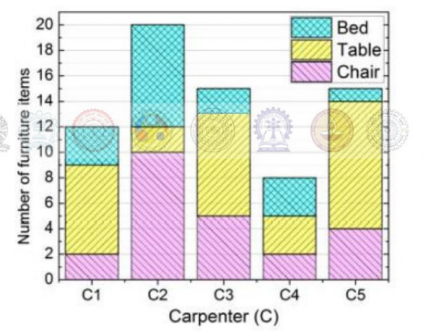
\includegraphics[width=0.5\textwidth]{figures/10.png}
\end{center}

\begin{enumerate}
    \item[(A)] Only i  
    \item[(B)] Only ii  
    \item[(C)] Both i and ii  
    \item[(D)] Neither i nor ii  
\end{enumerate}
\vspace{0.5cm}

\section*{Technical Section}

\questiona{The value of \( \lim\limits_{x \to 0} x \) is}{1}
\vspace{0.5cm}

\questiona{The real part of \( 6e^{i\pi/3} \) is}{2}

\vspace{0.5cm}

\questiona{The number of positive roots of the function \( f(x) \) shown below in the range \( 0 < x < 6 \) is}{3}
\begin{center}
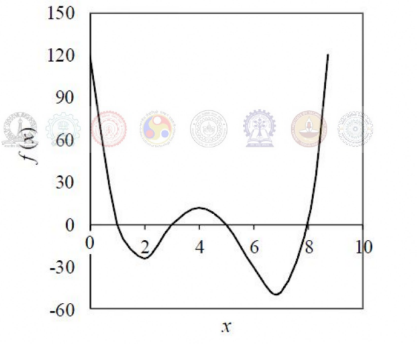
\includegraphics[width=0.5\textwidth]{figures/3.png}
\end{center}

\vspace{0.5cm}

\questiona{Let \( \mathbf{i} \) and \( \mathbf{j} \) be the unit vectors in the \( x \) and \( y \) directions, respectively. For the function \( F(x,y) = x^3 + y^2 \), the gradient of the function, i.e., \( \nabla F \), is given by}{4}
\begin{enumerate}
    \item[(A)] \( 3x^2\mathbf{i} - 2y\mathbf{j} \)  
    \item[(B)] \( 6x^2y \)  
    \item[(C)] \( 3x^2\mathbf{i} + 2y\mathbf{j} \)  
    \item[(D)] \( 2y\mathbf{i} - 3x^2\mathbf{j} \)  
\end{enumerate}
\vspace{0.5cm}

\questiona{The marks obtained by a set of students are: 38, 84, 45, 70, 75, 60, 48. \\ The mean and median marks, respectively, are}{5}
\begin{enumerate}
    \item[(A)] 45 and 75  
    \item[(B)] 55 and 48  
    \item[(C)] 60 and 60  
    \item[(D)] 60 and 70  
\end{enumerate}
\vspace{0.5cm}

\questiona{The volumetric properties of two gases M and N are described by the generalized compressibility chart which expresses the compressibility factor (Z) as a function of reduced pressure and reduced temperature only. The operating pressure (P) and temperature (T) of two gases M and N along with their critical properties (\( P_c, T_c \)) are given in the table below. \\

\begin{center}
\begin{tabular}{|c|c|c|c|c|}
\hline
Gas & \( P \) (bar) & \( T \) (K) & \( P_c \) (bar) & \( T_c \) (K) \\
\hline
M & 25 & 300 & 75 & 150 \\
N & 75 & 1000 & 225 & 500 \\
\hline
\end{tabular}
\end{center}

\( Z_M \) and \( Z_N \) are the compressibility factors of gases M and N under the given operating conditions, respectively. The relation between \( Z_M \) and \( Z_N \) is}{6}
\begin{enumerate}
    \item[(A)] \( Z_M = 8Z_N \)  
    \item[(B)] \( Z_N = 32Z_M \)  
    \item[(C)] \( Z_M = Z_N \)  
    \item[(D)] \( Z_N = 0.333Z_M \)  
\end{enumerate}
\vspace{0.5cm}

\questiona{Water is heated at atmospheric pressure from 40°C to 80°C using two different processes. In process I the heating is done by a source at 80°C. In process II, the water is first heated from 40°C to 60°C by a source at 60°C, and then from 60°C to 80°C by another source at 80°C. \\ Identify the correct statement.}{7}
\begin{enumerate}
    \item[(A)] Enthalpy change of water in process I is greater than enthalpy change in process II  
    \item[(B)] Enthalpy change of water in process II is greater than enthalpy change in process I  
    \item[(C)] Process I is closer to reversibility  
    \item[(D)] Process II is closer to reversibility  
\end{enumerate}
\vspace{0.5cm}

\questiona{In a venturi meter, \( \Delta P_1 \) and \( \Delta P_2 \) are the pressure drops corresponding to volumetric flow rates \( Q_1 \) and \( Q_2 \). If \( Q_2/Q_1 = 2 \), then \( \Delta P_2 / \Delta P_1 \) equals}{8}
\begin{enumerate}
    \item[(A)] 2  
    \item[(B)] 4  
    \item[(C)] 0.5  
    \item[(D)] 0.25  
\end{enumerate}
\vspace{0.5cm}

\questiona{The thickness of laminar boundary layer over a flat plate varies along the distance from the leading edge of the plate. As the distance increases, the boundary layer thickness}{9}
\begin{enumerate}
    \item[(A)] increases  
    \item[(B)] decreases  
    \item[(C)] initially increases and then decreases  
    \item[(D)] initially decreases and then increases  
\end{enumerate}
\vspace{0.5cm}

\questiona{Which of the following is the correct sequence of equipment for size reduction of solids?}{10}
\begin{enumerate}
    \item[(A)] Fluid energy mill \( \rightarrow \) Hammer mill \( \rightarrow \) Jaw crusher  
    \item[(B)] Hammer mill \( \rightarrow \) Jaw crusher \( \rightarrow \) Fluid energy mill  
    \item[(C)] Fluid energy mill \( \rightarrow \) Jaw crusher \( \rightarrow \) Hammer mill  
    \item[(D)] Jaw crusher \( \rightarrow \) Hammer mill \( \rightarrow \) Fluid energy mill  
\end{enumerate}
\vspace{0.5cm}

\questiona{A gas bubble (gas density \( \rho_g = 2 \,\mathrm{kg/m^3} \); bubble diameter \( D = 10^{-3} \,\mathrm{m} \)) is rising vertically through water (density \( \rho = 1000 \,\mathrm{kg/m^3} \); viscosity \( \mu = 0.001 \,\mathrm{Pa{\cdot}s} \)). Force balance on the bubble leads to an equation 
\begin{center}
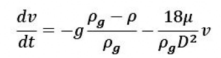
\includegraphics[width=0.4\textwidth]{figures/11.png}
\end{center}
where \( v \) is the velocity of the bubble at any given time \( t \). Assume that the volume of the rising bubble does not change. Take \( g = 9.81 \,\mathrm{m/s^2} \). \\ The terminal rising velocity of the bubble (in cm/s), rounded to 2 decimal places, is}{11}
\vspace{0.5cm}

\questiona{The one-dimensional unsteady heat conduction equation is  
\[
\frac{\partial T}{\partial t} = \alpha \left( \frac{1}{r^n} \frac{\partial}{\partial r} \left( r^n \frac{\partial T}{\partial r} \right) \right)
\]  
where \( T \) is temperature, \( t \) is time, \( r \) is radial position, \( k \) is thermal conductivity, \( \rho \) is density, and \( C_p \) is specific heat. \\  
For the cylindrical coordinate system, the value of \( n \) in the above equation is}{12}
\begin{enumerate}
    \item[(A)] 0  
    \item[(B)] 1  
    \item[(C)] 2  
    \item[(D)] 3  
\end{enumerate}
\vspace{0.5cm}

\questiona{In a heat exchanger, the inner diameter of a tube is 25 mm and its outer diameter is 30 mm. The overall heat transfer coefficient based on the inner area is 360 \( \mathrm{W/m^2{\cdot}^\circ C} \). \\  
Then, the overall heat transfer coefficient based on the outer area, rounded to the nearest integer, is \( \mathrm{W/m^2{\cdot}^\circ C} \).}{13}
\vspace{0.5cm}

\questiona{Which of the following conditions are valid at the plait point?  
\\ P) Density difference between the extract and raffinate phases is zero  
\\ Q) Interfacial tension between the extract and raffinate phases is zero  
\\ R) Composition difference between the extract and raffinate phases is zero}{14}
\begin{enumerate}
    \item[(A)] P and Q only  
    \item[(B)] Q and R only  
    \item[(C)] P and R only  
    \item[(D)] P, Q and R  
\end{enumerate}
\vspace{0.5cm}

\questiona{The composition of vapour entering a tray in a distillation column is 0.47. The average composition of the vapour leaving the tray is 0.53. The equilibrium composition of the vapour corresponding to the liquid leaving this tray is 0.52. All compositions are expressed in mole fraction of the more volatile component. \\  
The Murphree efficiency based on the vapour phase, rounded to the nearest integer, is \%.}{15}
\vspace{0.5cm}

\questiona{Consider steady state mass transfer of a solute A from a gas phase to a liquid phase. The gas phase bulk and interface mole fractions are \( y_{AG} \) and \( y_{Ai} \), respectively. The liquid phase bulk and interface mole fractions are \( x_{Ai} \) and \( x_{AL} \), respectively. The ratio  
\[
\frac{x_{Ai} - x_{AL}}{y_{AG} - y_{Ai}}
\]  
is very close to zero. \\  
This implies that mass transfer resistance is}{16}
\begin{enumerate}
    \item[(A)] negligible in the gas phase only  
    \item[(B)] negligible in the liquid phase only  
    \item[(C)] negligible in both the phases  
    \item[(D)] considerable in both the phases  
\end{enumerate}
\vspace{0.5cm}

\questiona{The following reaction rate curve is shown for a reaction \( A \rightarrow P \). Here, \( (-r_A) \) and \( X_A \) represent reaction rate and conversion, respectively. The feed is pure A and 90\% conversion is desired. \\  
Which amongst the following reactor configurations gives the lowest total volume of the reactor(s)?}{17}
\begin{center}
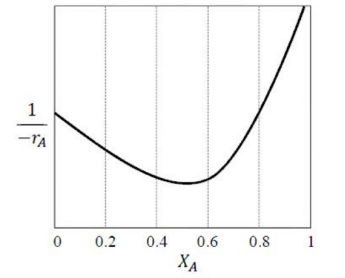
\includegraphics[width=0.5\textwidth]{figures/17.png}
\end{center}
\begin{enumerate}
    \item[(A)] CSTR followed by PFR  
    \item[(B)] Two CSTRs in series  
    \item[(C)] PFR followed by CSTR  
    \item[(D)] A single PFR  
\end{enumerate}
\vspace{0.5cm}

\questiona{Consider a first-order catalytic reaction in a porous catalyst pellet. Given:  
\\ \( R \): characteristic length of the pellet  
\\ \( D_e \): effective diffusivity  
\\ \( k_c \): mass transfer coefficient  
\\ \( k_1 \): rate constant based on volume of the catalyst pellet  
\\ \( C_s \): concentration of reactant on the pellet surface. \\  
The expression for Thiele modulus is}{18}
\begin{enumerate}
    \item[(A)] \( \dfrac{k_c R}{D_e} \)  
    \item[(B)] \( R \sqrt{\dfrac{k_1}{D_e}} \)  
    \item[(C)] \( \dfrac{D_e}{k_1 C_s} \)  
    \item[(D)] \( R \sqrt{\dfrac{1}{k_1}} \)  
\end{enumerate}
\vspace{0.5cm}

\questiona{For a solid-catalyzed gas phase reversible reaction, which of the following statements is ALWAYS TRUE?}{19}
\begin{enumerate}
    \item[(A)] Adsorption is rate-limiting  
    \item[(B)] Desorption is rate-limiting  
    \item[(C)] Solid catalyst does not affect equilibrium conversion  
    \item[(D)] Temperature does not affect equilibrium conversion  
\end{enumerate}
\vspace{0.5cm}

\questiona{Match the variables in Group-1 with the instruments in Group-2.  
\\ Group-1: P) Temperature Q) Liquid level R) Vacuum S) Concentration  
\\ Group-2: I) Capacitance probe II) McLeod gauge III) Chromatograph IV) Thermistor  
\\ Choose the correct set of combinations.}{20}
\begin{enumerate}
    \item[(A)] P-IV, Q-III, R-II, S-I  
    \item[(B)] P-I, Q-II, R-IV, S-III  
    \item[(C)] P-IV, Q-I, R-II, S-III  
    \item[(D)] P-III, Q-II, R-I, S-IV  
\end{enumerate}
\vspace{0.5cm}

\questiona{An LVDT (Linear Variable Differential Transformer) is a transducer used for converting}{21}
\begin{enumerate}
    \item[(A)] displacement to voltage  
    \item[(B)] voltage to displacement  
    \item[(C)] resistance to voltage  
    \item[(D)] voltage to current  
\end{enumerate}
\vspace{0.5cm}

\questiona{The cost of a new pump (including installation) is 24,000 Rupees. The pump has a useful life of 10 years. Its salvage value is 4,000 Rupees. Assuming straight line depreciation, the book value of the pump at the end of 4 years, rounded to the nearest integer, is Rupees.}{22}
\vspace{0.5cm}

\questiona{The DCDA (Double Contact Double Absorption) process is used for the manufacture of}{23}
\begin{enumerate}
    \item[(A)] urea  
    \item[(B)] sulphuric acid  
    \item[(C)] nitric acid  
    \item[(D)] ammonia  
\end{enumerate}
\vspace{0.5cm}

\questiona{Match the polymerization processes in Group-1 with the polymers in Group-2.  
\\ Group-1: P) Free radical polymerization Q) Ziegler Natta polymerization R) Condensation polymerization  
\\ Group-2: I) Nylon 6,6 II) Polypropylene III) Poly vinyl chloride  
\\ Choose the correct set of combinations.}{24}
\begin{enumerate}
    \item[(A)] P-I, Q-II, R-III  
    \item[(B)] P-II, Q-I, R-I  
    \item[(C)] P-I, Q-II, R-II  
    \item[(D)] P-II, Q-I, R-III  
\end{enumerate}
\vspace{0.5cm}

\questiona{The purpose of methanation reaction used in ammonia plants is to}{25}
\begin{enumerate}
    \item[(A)] remove CO as it is a catalyst poison  
    \item[(B)] increase the amount of hydrogen  
    \item[(C)] remove sulphur as it is a catalyst poison  
    \item[(D)] utilize methane as a catalyst for ammonia synthesis  
\end{enumerate}
\vspace{0.5cm}

\questionb{For the initial value problem  
\[
\frac{dx}{dt} = \sin(t), \quad x(0) = 0
\]  
the value of \( x \) at \( t = \frac{\pi}{3} \) is}{26}
\vspace{0.5cm}

\questionb{The Laplace transform of a function is  
\[
\frac{s+1}{s(s+2)}
\]  
The initial and final values, respectively, of the function are}{27}
\begin{enumerate}
    \item[(A)] 0 and 1  
    \item[(B)] 1 and 5  
    \item[(C)] \( \frac{1}{2} \) and 1  
    \item[(D)] \( \frac{1}{2} \) and 0  
\end{enumerate}
\vspace{0.5cm}

\questionb{Match the problem type in Group-1 with the numerical method in Group-2.  
\\ Group-1: P) System of linear algebraic equations Q) Non-linear algebraic equations R) Ordinary differential equations S) Numerical integration  
\\ Group-2: I) Newton-Raphson II) Gauss-Seidel III) Simpson’s rule IV) Runge-Kutta  
\\ Choose the correct set of combinations.}{28}
\begin{enumerate}
    \item[(A)] P-II, Q-I, R-III, S-IV  
    \item[(B)] P-I, Q-II, R-IV, S-III  
    \item[(C)] P-IV, Q-III, R-II, S-I  
    \item[(D)] P-II, Q-I, R-IV, S-III  
\end{enumerate}
\vspace{0.5cm}

\questionb{A box has 6 red balls and 4 white balls. A ball is picked at random and replaced in the box, after which a second ball is picked. \\  
The probability of both the balls being red, rounded to 2 decimal places, is}{29}
\vspace{0.5cm}

\questionb{An aqueous salt solution enters a crystallizer operating at steady state at 25°C. The feed temperature is 90°C and the salt concentration in the feed is 40 weight \%. The salt crystallizes as a pentahydrate. The crystals and the mother liquor leave the crystallizer. The molecular weight of the anhydrous salt is 135. The solubility of the salt at 25°C is 20 weight \%. \\  
The feed flowrate required for a production rate of 100 kg/s of the hydrated salt, rounded to the nearest integer, is kg/s.}{30}
\vspace{0.5cm}

\questionb{Reaction \( A \rightarrow B \) is carried out in a reactor operating at steady state and 1 mol/s of pure A at 425°C enters the reactor. The outlet stream leaves the reactor at 325°C. The heat input to the reactor is 17 kW. The heat of reaction at the reference temperature of 25°C is 30 kJ/mol. The specific heat capacities (in kJ/mol.K) of A and B are 0.1 and 0.15, respectively. \\  
The molar flowrate of B leaving the reactor, rounded to 2 decimal places, is mol/s.}{31}
\vspace{0.5cm}

\questionb{The pressure of a liquid is increased isothermally. The molar volume of the liquid decreases from \( 50.45 \times 10^{-6} \,\mathrm{m^3/mol} \) to \( 48 \times 10^{-6} \,\mathrm{m^3/mol} \). The isothermal compressibility of the liquid is \( 10^{-9} \,\mathrm{Pa^{-1}} \), which can be assumed to be independent of pressure. \\  
The change in the molar Gibbs free energy of the liquid, rounded to nearest integer, is J/mol.}{32}
\vspace{0.5cm}

\questionb{A sparingly soluble gas (solute) is in equilibrium with a solvent at 10 bar. The mole fraction of the solute in the gas phase is 0.01. At the operating temperature and pressure, the fugacity coefficient of the solute in the gas phase and the Henry's law constant are 0.92 and 1000 bar, respectively. Assume that the liquid phase obeys Henry’s law. \\  
The mole percentage of the solute in the liquid phase, rounded to 2 decimal places, is}{33}
\vspace{0.5cm}

\questionb{The vapour pressure of a pure substance at a temperature \( T \) is 30 bar. The actual and ideal gas values of \( g/RT \) for the saturated vapour at this temperature \( T \) and 30 bar are 7.0 and 7.7, respectively. Here, \( g \) is the molar Gibbs free energy and \( R \) is the universal gas constant. \\  
The fugacity of the saturated liquid at these conditions, rounded to 1 decimal place, is bar.}{34}
\vspace{0.5cm}

\questionb{Oil is being delivered at a steady flowrate through a circular pipe of radius \( 1.25 \times 10^{-2} \,\mathrm{m} \) and length 10 m. The pressure drop across the pipe is 500 Pa. \\  
The shear stress at the pipe wall, rounded to 2 decimal places, is Pa.}{35}
\vspace{0.5cm}

\questionb{The following table provides four sets of Fanning friction factor data for different values of Reynolds number (Re) and roughness factor \( \frac{k}{D} \):  
\begin{center}
\begin{tabular}{|c|c|c|c|c|}
\hline
Set & Re = \(10^3\) & \(10^4\) & \(10^5\) & \(10^6\) \\
\hline
I & 0.16 & 0.016 & \( \frac{16}{10^4} \) & \( \frac{16}{10^5} \) \\
II & 0.016 & 0.16 & 0.0055 & 0.0045 \\
III & 0.16 & 0.016 & 0.0045 & 0.0055 \\
IV & 0.0045 & 0.0055 & 0.016 & 0.16 \\
\hline
\end{tabular}
\end{center}
Which of the above sets of friction factor data is correct?}{36}
\begin{enumerate}
    \item[(A)] Set I  
    \item[(B)] Set II  
    \item[(C)] Set III  
    \item[(D)] Set IV  
\end{enumerate}
\vspace{0.5cm}

\questionb{A propeller (diameter \( D = 15 \) m) rotates at \( N = 1 \) revolution per second. To understand the flow around the propeller, a lab-scale model is made. Important parameters to study the flow are velocity of the propeller tip (\( V = \pi ND \)), diameter \( D \), and acceleration due to gravity \( g \). The lab-scale model is \( \frac{1}{100}^{th} \) the size of the actual propeller. \\  
The rotation speed of the lab-scale model, to the nearest integer, should be rev/s.}{37}
\vspace{0.5cm}

\questionb{Size analysis was carried out on a sample of gravel. The data for mass fraction (\( x_i \)) and average particle diameter (\( D_{pi} \)) of the fraction is given below:

\begin{center}
\begin{tabular}{|c|c|}
\hline
\( x_i \) & \( D_{pi} \) (mm) \\
\hline
0.2 & 5 \\
0.4 & 10 \\
0.4 & 20 \\
\hline
\end{tabular}
\end{center}
The mass mean diameter of the sample, to the nearest integer, is mm.}{38}
\vspace{0.5cm}

\questionb{Let \( I_{b\lambda} \) be the spectral blackbody radiation intensity per unit wavelength about the wavelength \( \lambda \). \\  
The blackbody radiation intensity emitted by a blackbody over all wavelengths is}{39}
\begin{center}
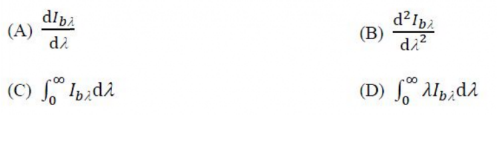
\includegraphics[width=0.7\textwidth]{figures/39.png}
\end{center}
\vspace{0.5cm}

\questionb{A fluid flows over a heated horizontal plate maintained at temperature \( T_w \). The bulk temperature of the fluid is \( T_m \). The temperature profile in the thermal boundary layer is given by:  
\[
T = T_w + (T_w - T_m) \left[ 2 \left( \frac{y}{\delta_t} \right) - \left( \frac{y}{\delta_t} \right)^3 \right], \quad 0 < y < \delta_t
\]  
Here, \( y \) is the vertical distance from the plate, \( \delta_t \) is the thickness of the thermal boundary layer, and \( k \) is the thermal conductivity of the fluid.  
\\ The local heat transfer coefficient is given by}{40}
\begin{enumerate}
    \item[(A)] \( \frac{k}{\delta_t} \)  
    \item[(B)] \( \frac{2k}{\delta_t} \)  
    \item[(C)] \( \frac{3k}{\delta_t} \)  
    \item[(D)] \( \frac{4k}{\delta_t} \)  
\end{enumerate}
\vspace{0.5cm}

\questionb{In nucleate boiling, the pressure inside a bubble is higher than the pressure of the surrounding liquid. Assuming that both the liquid and vapour are saturated, the temperature of the liquid will ALWAYS be}{41}
\begin{enumerate}
    \item[(A)] at 100 °C  
    \item[(B)] lower than the temperature of the vapour  
    \item[(C)] equal to the temperature of the vapour  
    \item[(D)] higher than the temperature of the vapour  
\end{enumerate}
\vspace{0.5cm}

\questionb{The vapor phase composition and relative volatilities (with respect to n-propane) on an ideal tray of a distillation column are:  
\begin{center}
\begin{tabular}{|c|c|c|}
\hline
Component & Mole fraction in vapour & Relative volatility \\
\hline
Methane & 0.12 & 10 \\
Ethane & 0.28 & 4 \\
n-Propane & 0.60 & 1 \\
\hline
\end{tabular}
\end{center}
The mole fraction of n-propane in the liquid phase, rounded to 2 decimal places, is}{42}
\vspace{0.5cm}

\questionb{The Sherwood number (Sh\textsubscript{L}) correlation for laminar flow over a flat plate of length \( L \) is given by  
\[
\text{Sh}_L = 0.664 \text{Re}_L^{1/2} \text{Sc}^{1/3}
\]  
where Re\textsubscript{L} and Sc represent Reynolds number and Schmidt number, respectively.  
This correlation, expressed in the form of Chilton-Colburn \( j_D \) factor, is}{43}
\begin{enumerate}
    \item[(A)] \( j_D = 0.664 \)  
    \item[(B)] \( j_D = 0.664 \text{Re}_L \text{Sc} \)  
    \item[(C)] \( j_D = 0.664 \text{Re}_L^{1/2} \)  
    \item[(D)] \( j_D = 0.664 \text{Re}_L^{-1/2} \text{Sc}^{1/3} \)  
\end{enumerate}
\vspace{0.5cm}

\questionb{In a countercurrent stripping operation using pure steam, the mole ratio of a solute in the liquid stream is reduced from 0.25 to 0.05. The liquid feed flowrate, on a solute-free basis, is 3 mol/s. The equilibrium line for the system is given in the figure below.  
\\ The minimum flowrate of pure steam for this process, rounded to 1 decimal place, is mol/s.}{44}
\begin{center}
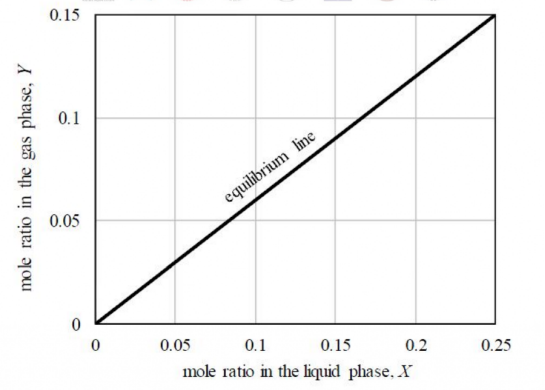
\includegraphics[width=0.5\textwidth]{figures/44.png}
\end{center}
\vspace{0.5cm}

\questionb{In a batch adsorption process, 5 g of fresh adsorbent is used to treat 1 liter of an aqueous phenol solution. The initial phenol concentration is 100 mg/liter. The equilibrium relation is given by  
\[
q^* = 13C
\]  
where \( q^* \) is the amount of phenol adsorbed in mg of phenol per gram of adsorbent, and \( C \) is the concentration of phenol in mg/liter in the aqueous solution.  
\\ When equilibrium is attained between the adsorbent and the solution, the concentration of phenol in the solution, rounded to 1 decimal place, is mg/liter.}{45}
\vspace{0.5cm}

\questionb{The C-curve measured during a pulse tracer experiment is shown below. In the figure, \( C(t) \) is the concentration of the tracer measured at the reactor exit in mol/liter at time \( t \) seconds.  
\\ The mean residence time in the reactor, rounded to 1 decimal place, is s.}{46}
\begin{center}
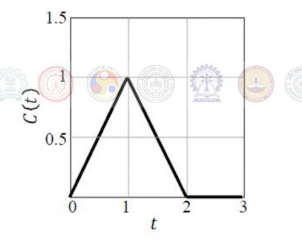
\includegraphics[width=0.5\textwidth]{figures/46.png}
\end{center}
\vspace{0.5cm}

\questionb{The following liquid phase second-order reaction is carried out in an isothermal CSTR at steady state:  
\[
A \rightarrow R, \quad (-r_A) = 0.005 C^2 \text{ mol/m}^3\cdot\text{hr}
\]  
The reactor volume is 2 m\textsuperscript{3}, the inlet flowrate is 0.5 m\textsuperscript{3}/hr, and the inlet concentration of the reactant is 1000 mol/m\textsuperscript{3}.  
\\ The fractional conversion, rounded to 2 decimal places, is}{47}
\vspace{0.5cm}

\questionb{The reversible reaction of t-butyl alcohol (TBA) and ethanol (EtOH) to ethyl t-butyl ether (ETBE) is  
\[
\text{TBA} + \text{EtOH} \rightleftharpoons \text{ETBE} + \text{Water}
\]  
The equilibrium constant for this reaction is \( K_{eq} = 1 \). Initially, 74 g of TBA is mixed with 100 g of aqueous solution containing 46 weight\% ethanol. The molecular weights are: TBA = 74, EtOH = 46, ETBE = 102, Water = 18.  
\\ The mass of ETBE at equilibrium, rounded to 1 decimal place, is g.}{48}
\vspace{0.5cm}

\questionb{The following gas-phase reaction is carried out in a constant-volume isothermal batch reactor:  
\[
A + B \rightarrow R + S
\]  
The reactants A and B as well as product S are non-condensable gases. At the operating temperature, the saturation pressure of the product R is 40 kPa.  
\\ Initially, the batch reactor contains equimolar amounts of A and B (no products) at a total pressure of 100 kPa. The initial concentrations of the reactants are \( C_{A0} = C_{B0} = 12.5 \) mol/m\textsuperscript{3}. The rate of reaction is given by \( -r_A = 0.08 C_A C_B \text{ mol/m}^3\cdot s \).  
\\ The time at which R just starts condensing, rounded to 1 decimal place, is s.}{49}
\vspace{0.5cm}

\questionb{The transfer function of a system is  
\[
\frac{1}{4s^2 + 12s + 1}
\]  
For a unit step increase in the input, the fractional overshoot, rounded to 2 decimal places, is}{50}
\vspace{0.5cm}

\questionb{The open loop transfer function of a process with a proportional controller (gain \( K_c \)) is  
\[
G_{OL} = \frac{K_c e^{-2s}}{s}
\]  
Based on the Bode criterion for closed-loop stability, the ultimate gain of the controller, rounded to 2 decimal places, is}{51}
\vspace{0.5cm}

\questionb{The characteristic equation of a closed-loop system is  
\[
6s^3 + 11s^2 + 6s + (1 + K) = 0, \quad \text{where } K > 0
\]  
The value of \( K \) beyond which the system just becomes unstable, rounded to the nearest integer, is}{52}
\vspace{0.5cm}

\questionb{A bond has a maturity value of 20,000 Rupees at the end of 4 years. The interest is compounded at the rate of 5\% per year.  
\\ The initial investment to be made, rounded to the nearest integer, is Rupees.}{53}
\vspace{0.5cm}

\questionb{The total cost (\( C_T \)) of an equipment in terms of the operating variables \( x \) and \( y \) is  
\[
C_T = 2x + \frac{2000}{x} + y + 5
\]  
The optimal value of \( C_T \), rounded to 1 decimal place, is}{54}
\vspace{0.5cm}

\questionb{Match the equipment in Group-1 with the process in Group-2.  
\\ Group-1: P) Fluidized bed Q) Multistage adiabatic reactor with inter-stage cooling R) Fourdrinier machine S) Diaphragm cell  
\\ Group-2: I) Paper-making II) Sodium hydroxide manufacture III) SO\textsubscript{2} oxidation IV) Catalytic cracking  
\\ Choose the correct set of combinations.}{55}
\begin{enumerate}
    \item[(A)] P-IV, Q-III, R-I, S-II  
    \item[(B)] P-IV, Q-III, R-II, S-I  
    \item[(C)] P-III, Q-IV, R-I, S-II  
    \item[(D)] P-III, Q-IV, R-II, S-I  
\end{enumerate}
\vspace{0.5cm}
\vspace{5cm}
\begin{center}
\textbf{END OF THE QUESTION PAPER} \\
\rule{\textwidth}{0.5pt}
\end{center}


\end{document}